\section{Korrelationsmatrizen sortiert nach dem Gemeindeschlüssel}
\subsection{Landkreise}
In \autoref{fig:matrizes_north_to_south_counties} finden sich die sechs Matrizen mit den Werten für die Korrelationen zwischen den Landkreisen.
Die Zeilen und Spalten sind lexikographisch nach den Gemeindeschlüsseln der Landkreise sortiert, dies entspricht in etwa einem Nord-Süd-Verlauf (siehe \todo{Nord-Süd-verlauf Bild verlinken}. Eine vollständige Auflistung befindet sich im Anhang in \autoref{tab:counties_by_admunitid}.

\begin{figure}[H]
    \centering
    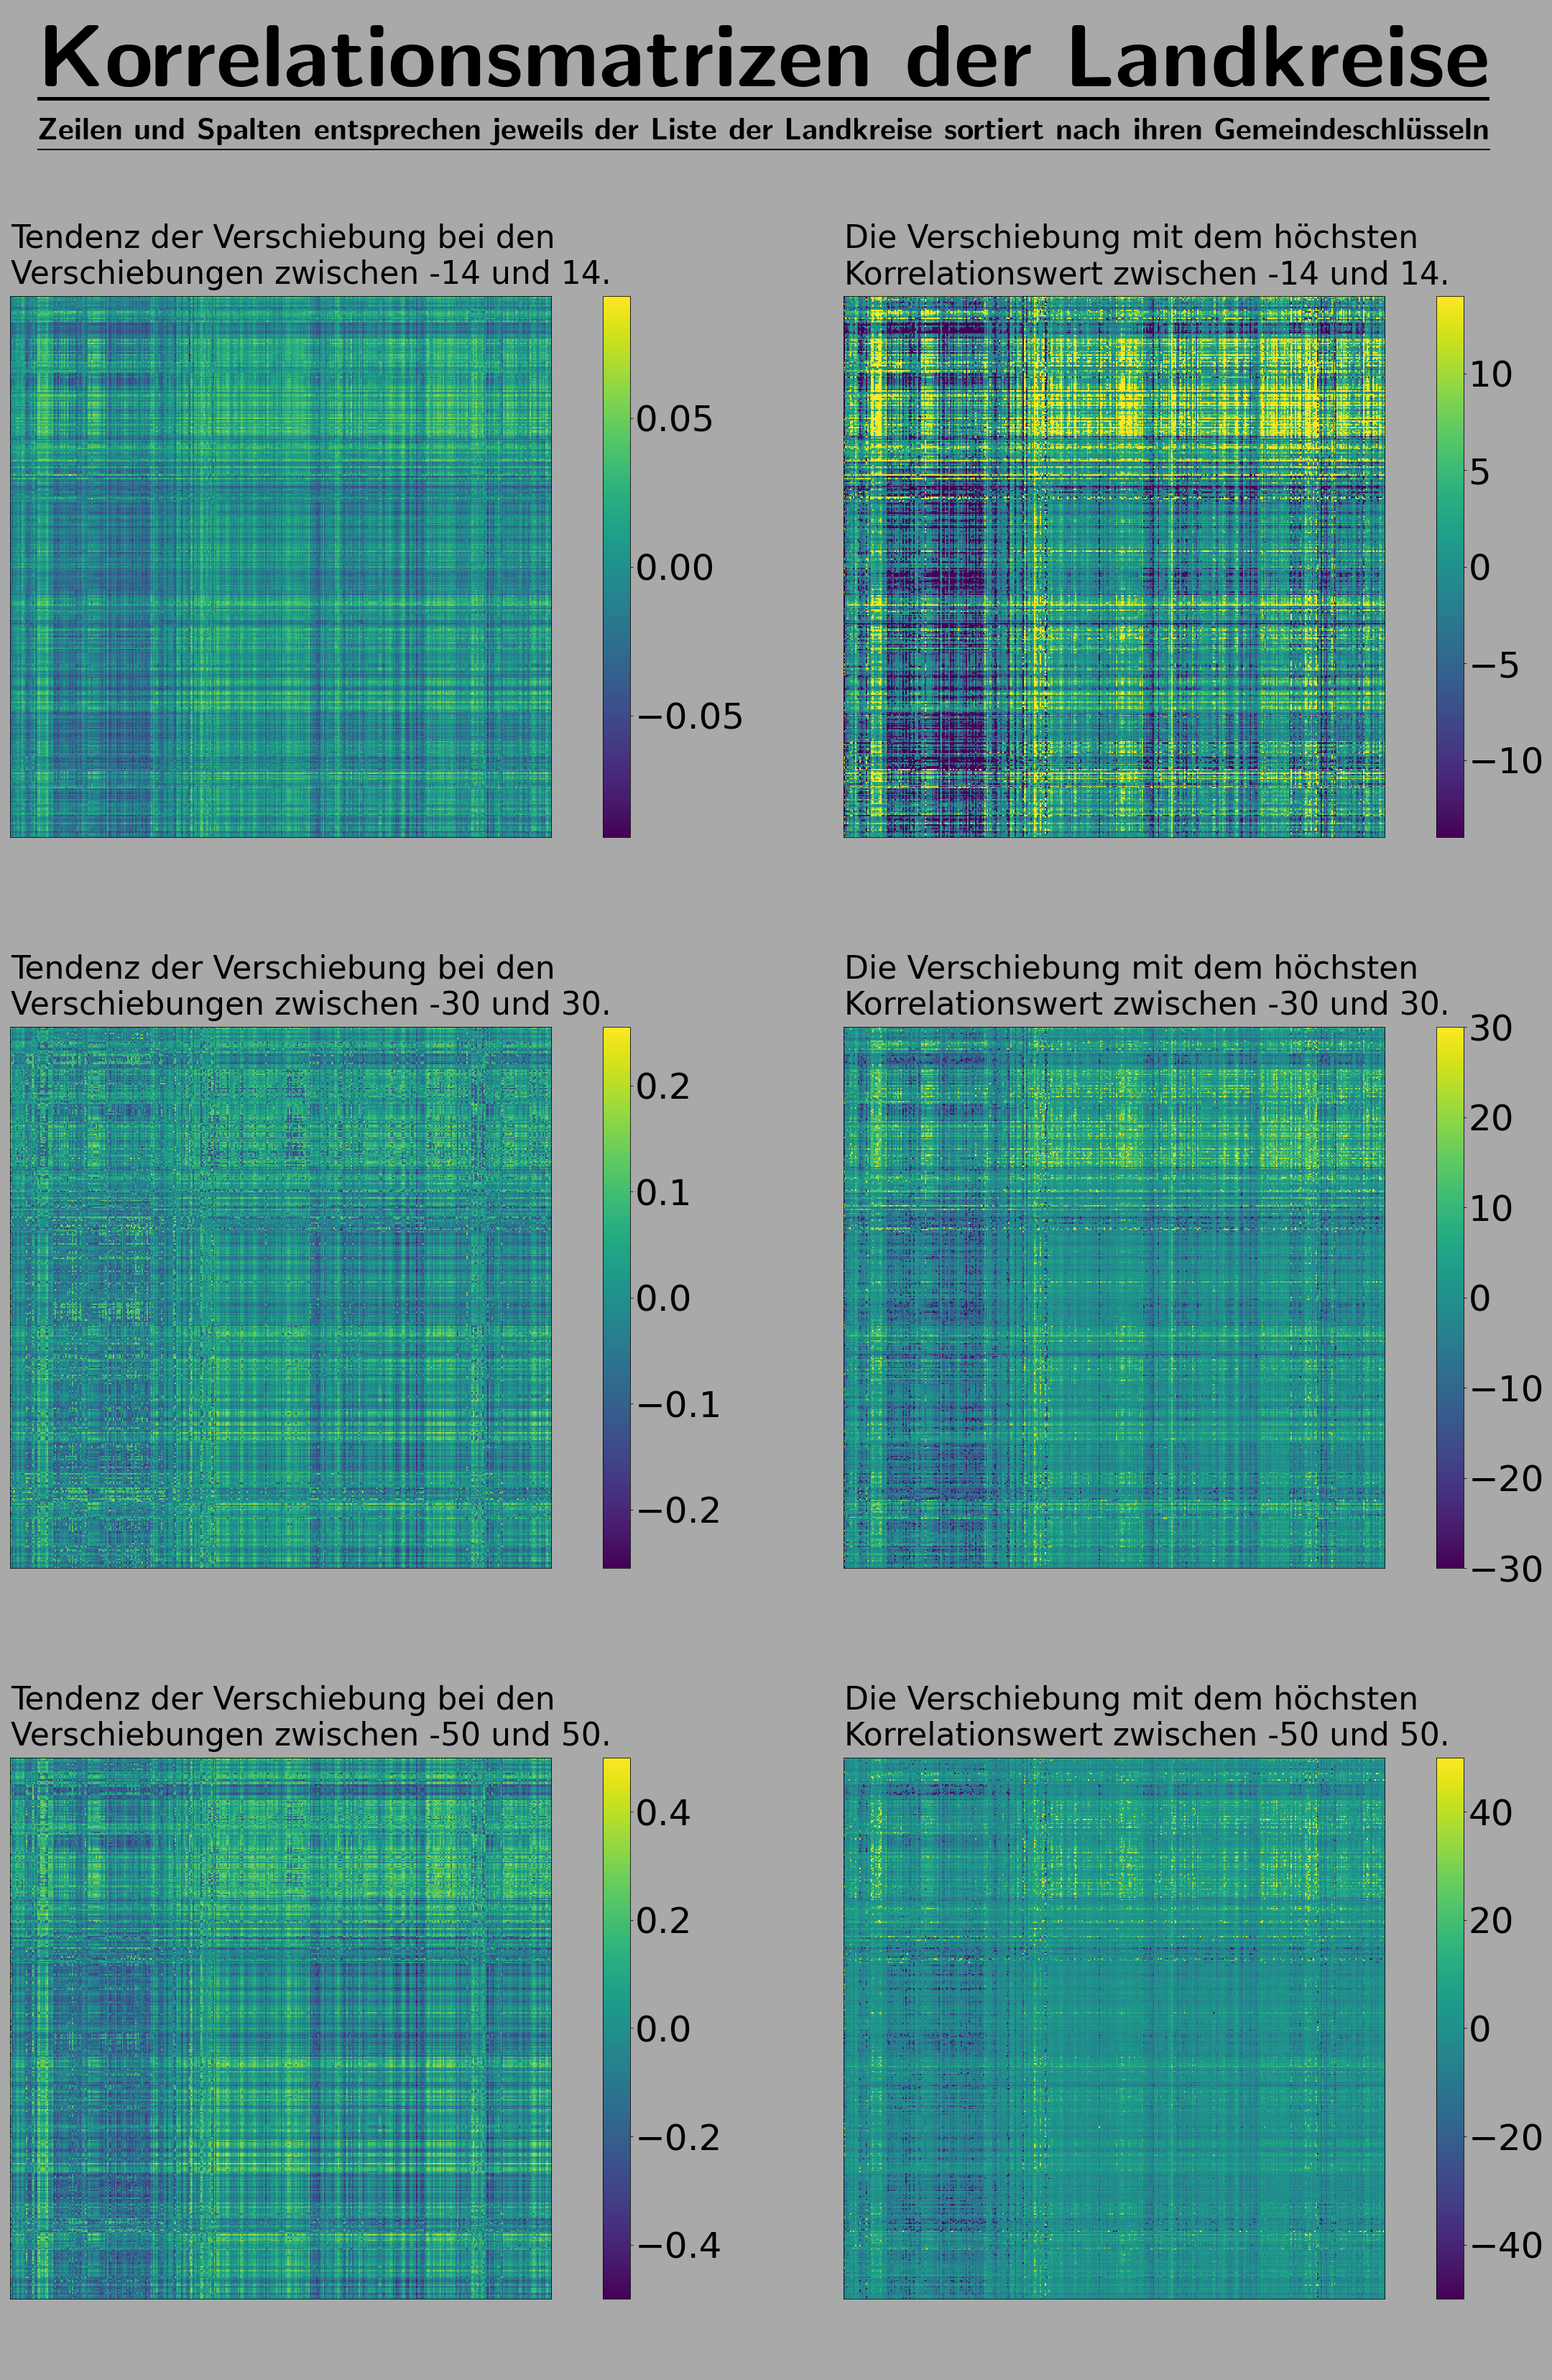
\includegraphics[width = 0.95\textwidth]{figures/Ergebnisse/matrizes_north_to_south_counties.png}
    \caption{Verschiedene Korrelationsmatrizen berechnet aus den Korrelationen jedes deutschen Landkreises mit sich selbst und jedem anderen deutschen Landkreis. Jeder Zeile und Spalte sind Landkreise zugeteilt, die vollständige Auflistung befindet sich im Anhang. Die Farben der Zellen auf der linken Seite entsprechen der Differenz zwischen der durchschnittlichen Korrelationswahrscheinlichkeit für negative Verschiebungen des Landkreises der Spalte in Relation zum Landkreis der Zeile und der durchschnittlichen Korrelationswahrscheinlichkeit für die zugehörigen positiven Verschiebungen.
    Auf der rechten Seite wir die Zelle entsprechend der Verschiebung der Zeitserie des Landkreises der Spalte entgegen der Zeitserie der Zeile mit der höchsten Korrelationswahrscheinlichkeit eingefärbt. Beide Vorgehensweise werden für alle ganzzahligen Verschiebungen $\tau\in[-14,14]$,  $\tau\in[-30,30]$ und  $\tau\in[-50,50]$ durchgeführt und in dieser Reihenfolge von oben nach unten dargestellt.}
    \label{fig:matrizes_north_to_south_counties}
\end{figure}

\todo{Richtige Richtung? Nachprüfen! (Spalte und Zeile evtl. tauschen)}

\subsection{Regierungsbezirke}
In \autoref{fig:matrizes_north_to_south_districts} finden sich die sechs Matrizen mit den Werten für die Korrelationen zwischen den Bezirken. Die Zeilen und Spalten sind lexikographisch nach den Gemeindeschlüsseln der Landkreise in den Regierungsbezirken sortiert, eine vollständige Auflistung befindet sich im Anhang in \autoref{tab:districts_by_admunitid}

\begin{figure}[H]
    \centering
    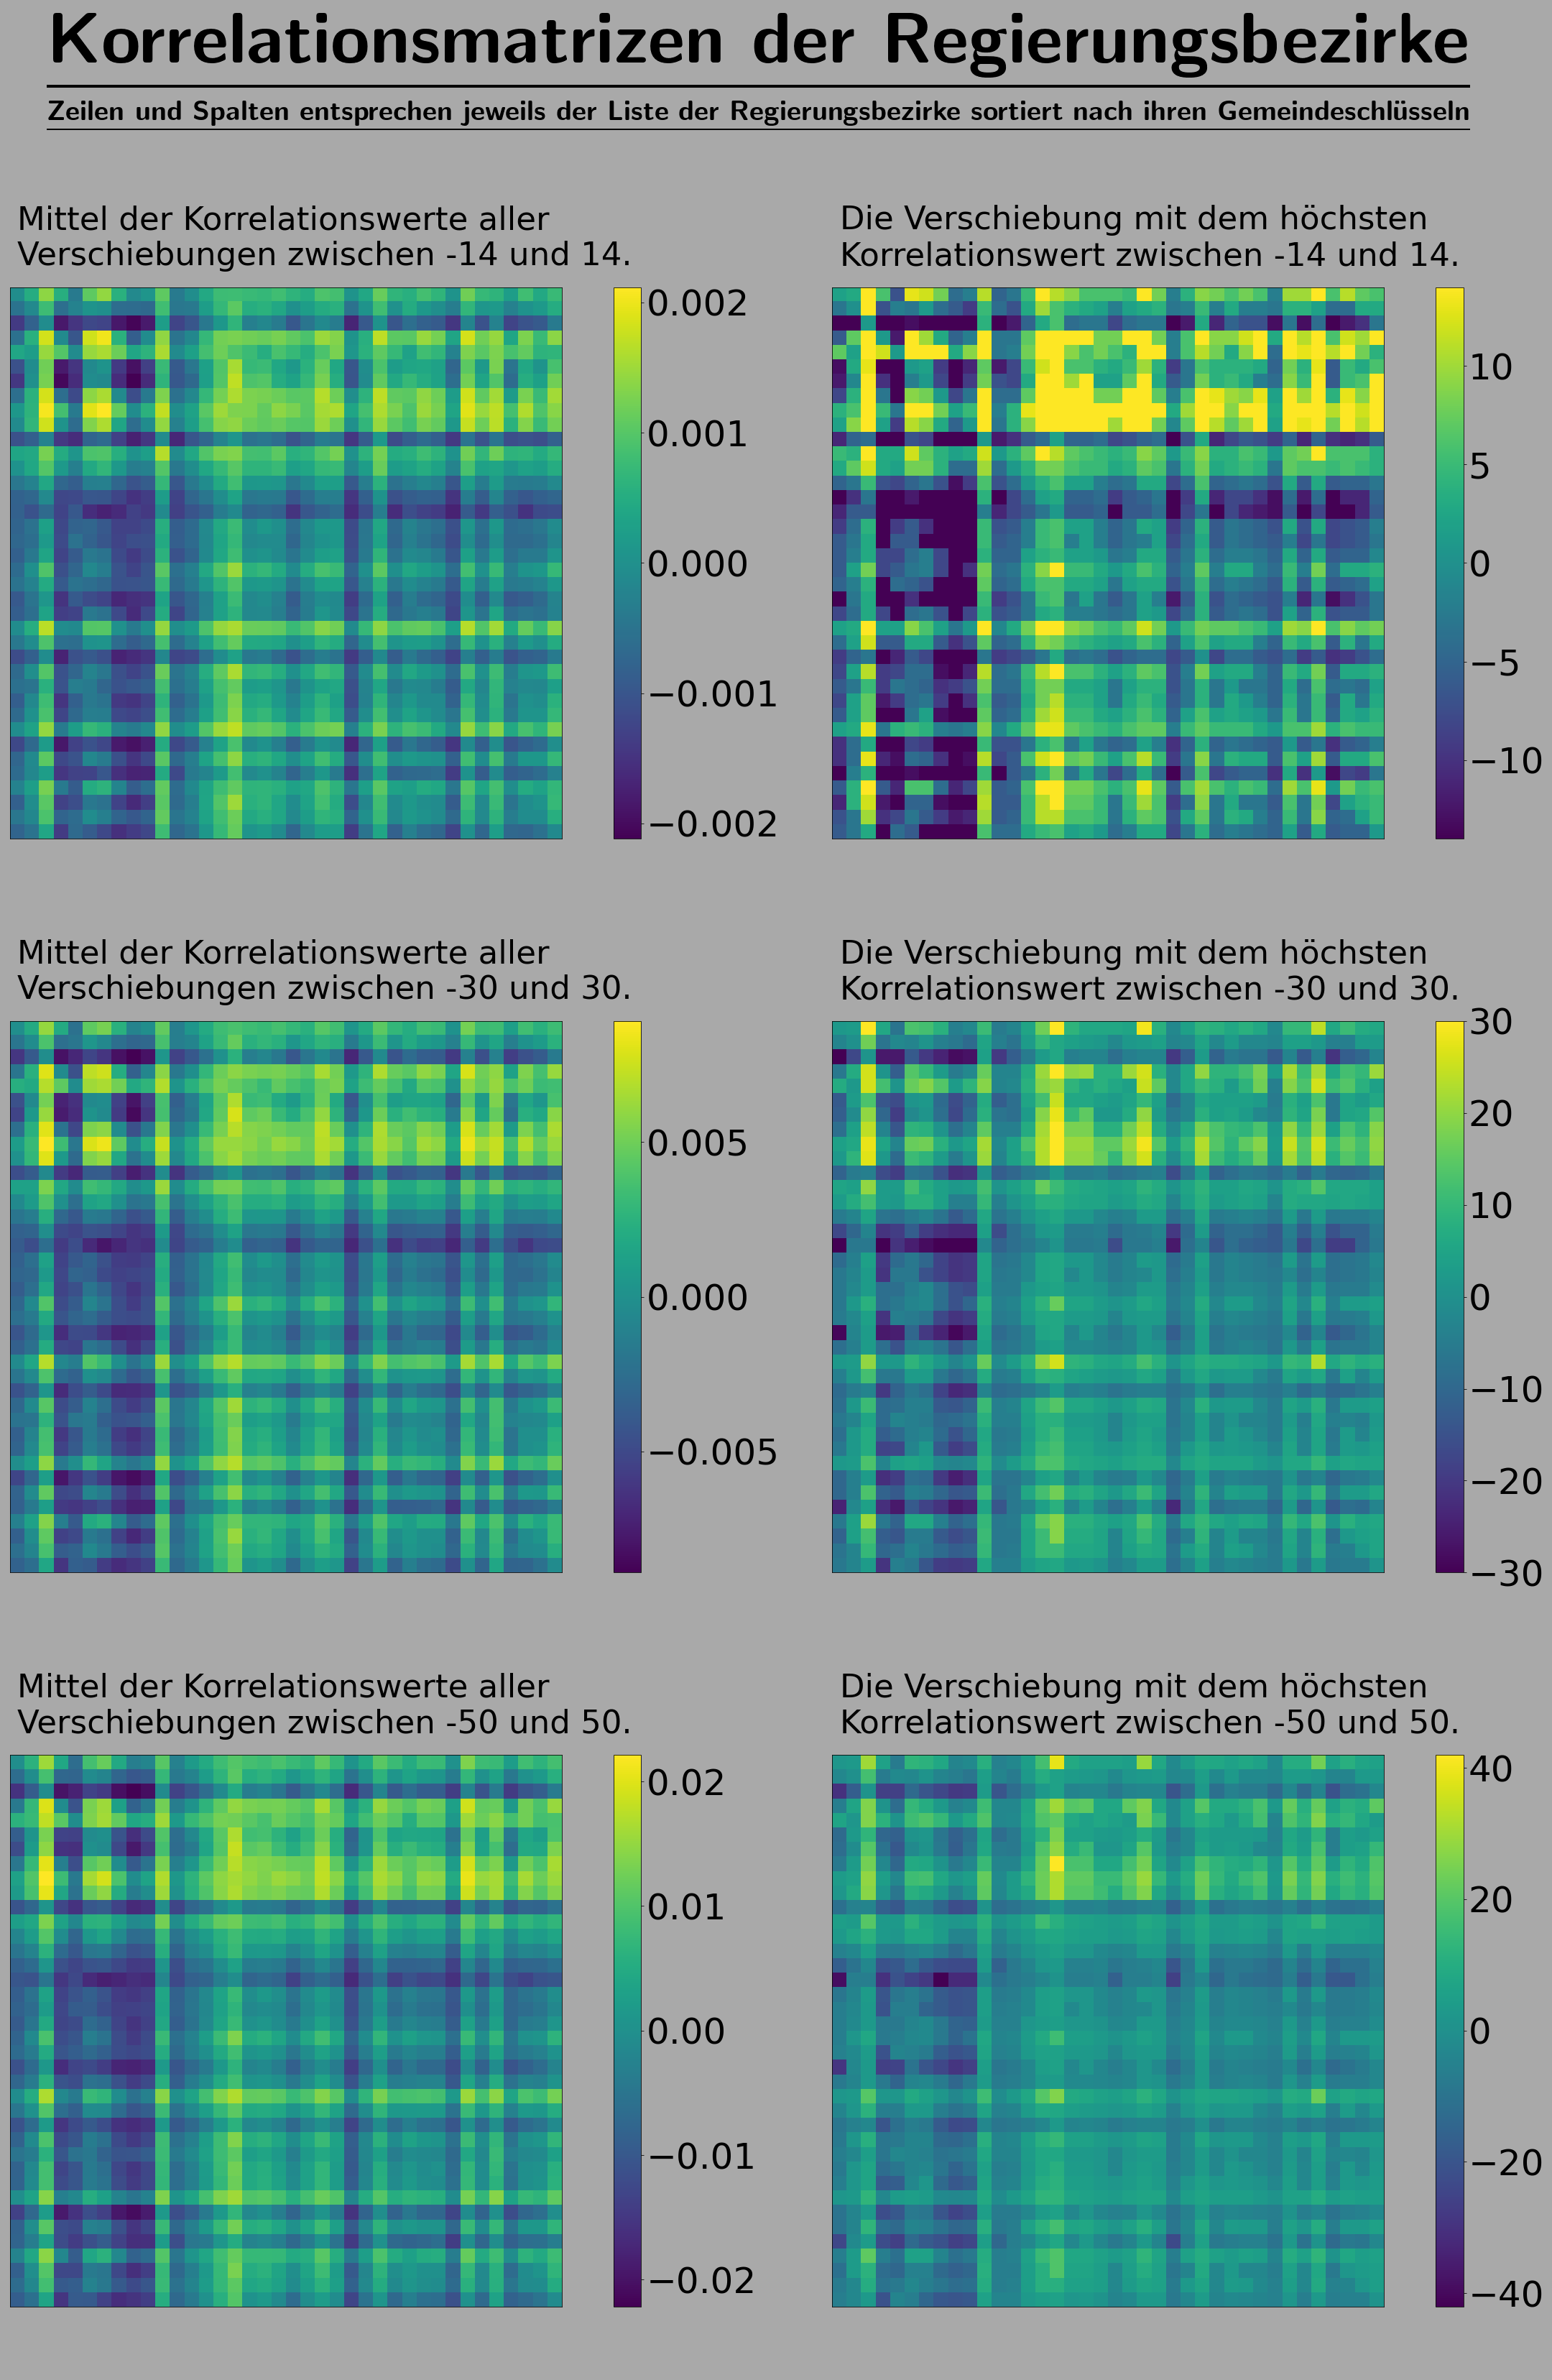
\includegraphics[width = 0.95\textwidth]{figures/Ergebnisse/matrizes_north_to_south_districts.png}
    \caption{Verschiedene Korrelationsmatrizen berechnet aus den Korrelationen jedes deutschen Regierungsbezirks mit sich selbst und jedem anderen deutschen Regierungsbezirks. Jeder Zeile und Spalte sind Regierungsbezirke zugeteilt, die vollständige Auflistung befindet sich im Anhang. Die Farben der Zellen auf der linken Seite entsprechen der Differenz zwischen der durchschnittlichen Korrelationswahrscheinlichkeit für negative Verschiebungen des Regierungsbezirks der Spalte in Relation zum Regierungsbezirk der Zeile und der durchschnittlichen Korrelationswahrscheinlichkeit für die zugehörigen positiven Verschiebungen.
    Auf der rechten Seite wir die Zelle entsprechend der Verschiebung der Zeitserie des Regierungsbezirks der Spalte entgegen der Zeitserie der Zeile mit der höchsten Korrelationswahrscheinlichkeit eingefärbt. Beide Vorgehensweise werden für alle ganzzahligen Verschiebungen $\tau\in[-14,14]$,  $\tau\in[-30,30]$ und  $\tau\in[-50,50]$ durchgeführt und in dieser Reihenfolge von oben nach unten dargestellt.}
    \label{fig:matrizes_north_to_south_districts}
\end{figure}
\todo{Richtige Richtung? Nachprüfen! (Spalte und Zeile evtl. tauschen)}
